\section{Problem set 2}
\subsection{Preface}
This problem set provided an introduction to simple pseudorandom number
generator called ,,linear-feedback shift register'' (LSFR) which is a shift
register whose input bit is a linear function of it's previous state. The goal
of this problem set was to get familiar with LSFR structure, analyze it's possible
input - initialization vector - and output generated using different IVs.

\subsection{Assignment 1}
The goal of this task was to analyze and sketch out architectures of the
\texttt{LSFR} entity provided by the lecturer. Figure \ref{fig:assignment1-lsfr_first}
is an analysis of \texttt{first} architecture with marked corresponding testbench
ports. Same analysis for \texttt{second} architecture is done on figure \ref{fig:assignment1-lsfr_second}.

\begin{figure}[!htb]
  \center{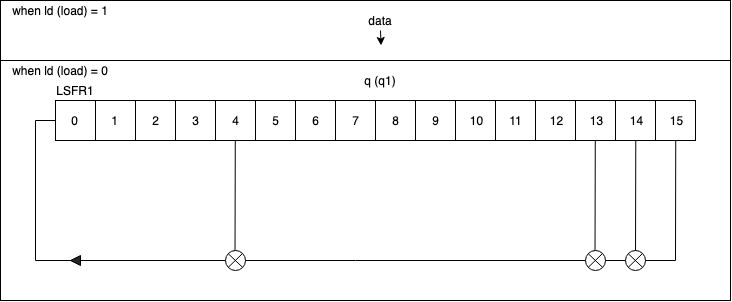
\includegraphics[scale=0.5]
  {drawings/lsfr_first.png}}
  \caption{\label{fig:assignment1-lsfr_first} Architecture \texttt{first} of \texttt{LSFR}.}
\end{figure}

\begin{figure}[!htb]
  \center{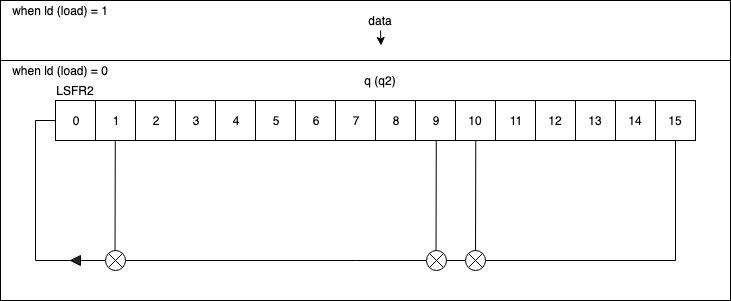
\includegraphics[scale=0.5]
  {drawings/lsfr_second.png}}
  \caption{\label{fig:assignment1-lsfr_second} Architecture \texttt{second} of \texttt{LSFR}.}
\end{figure}

\subsection{Assignment 2}

\subsection{Assignment 3}
The goal of this assignment was to create simulation of \texttt{A5/1} stream
cypher using \texttt{LSFR} entity from previous assignments. Basically,
\texttt{A5/1} is a construct that is a combination of three \texttt{LFSR}s
with different size - $q_1$ with size of 19 bits, $q_2$ of size 22 bits and
$q_3$ - 23 bits. Each of \texttt{LFSRs} outputs is combined using \texttt{XOR}
and the result of this operation is next number generated by \texttt{LFSR}.

To make output more random, authors of \texttt{A5/1} introduced idea of
\textit{majority voting}, that is, only \texttt{LFSR}s with value at specific
position being in majority gets shifted on clock event. For smallest
\texttt{LFSR} (with length of 19 bits), bit at the specific position is $8^{th}$
bit, for medium one (length of 22 bits) its $10^{th}$ bit and for the biggest
 (length of 23 bits) its also $10^{th}$ bit.

 Examples of majority voting:
 $q_1[8] = 1, q_2[10] = 1, g_3[10] = 1$ - major bit is $1$, so all $q$ move.
 $q_1[8] = 1, q_2[10] = 1, g_3[10] = 0$ - major bit is $1$, so $q_1$ and $q_2$ move.
 $q_1[8] = 0, q_2[10] = 1, g_3[10] = 0$ - major bit is $0$, so $q_1$ and $q_3$ move.

To implement \texttt{A5/1} with majority voting, I've decided to create a single
entity. Created entity contained of 4 ports, their definition is shown on
listing \ref{fig:assignment3-ports}. Port \texttt{clk} is for clock,
\texttt{ld} is a switch between loading state and working state,
\texttt{data} is a 64-bit initialization vector for \texttt{LSFR}s and
results is the only output signal that contains resulted pseudorandom number
generated by \texttt{A5/1}.

\begin{lstlisting}[
  style=vhdl,
  caption={\texttt{A5/1} ports definition},
  captionpos=b,
  label={fig:assignment3-ports}
]
  Port (
    clk : in std_logic;
    ld : in std_logic;
    data : in std_logic_vector(63 downto 0) := (others => '0');
    result : out std_logic
  );
\end{lstlisting}

Architecture of created \texttt{A5/1} entity contains 3 \texttt{std\_logic\_vector}
signals $q_1, q_2, q_3$ representing three \texttt{LSFR}s and \texttt{std\_logic}
signal used to store major bit. Part of architecture with signals definitions
is showed in listing \ref{fig:assignment3-signals}.

\begin{lstlisting}[
  style=vhdl,
  caption={\texttt{A5/1} signals definition},
  captionpos=b,
  label={fig:assignment3-signals}
]
  signal q1 : STD_LOGIC_VECTOR(18 downto 0) := (OTHERS => '0');
  signal q2 : STD_LOGIC_VECTOR(21 downto 0) := (OTHERS => '0');
  signal q3 : STD_LOGIC_VECTOR(22 downto 0) := (OTHERS => '0');
  signal major : STD_LOGIC;
\end{lstlisting}

Process definition contains if statement to differentiate between
loading phase and non-loading phase. During loading phase, when \texttt{ld = '1'},
initialization vector is being chunked and assigned to corresponding $q_i$
\texttt{LSFR}s. This phase is shown on listing \ref{fig:assignment3-iv-to-registers}.

\begin{lstlisting}[
  style=vhdl,
  caption={\texttt{A5/1} \texttt{IV} vector assigned to registers},
  captionpos=b,
  label={fig:assignment3-iv-to-registers}
]
  q1 <= data(18 downto 0);
  q2 <= data(40 downto 19);
  q3 <= data(63 downto 41);
\end{lstlisting}

After switching \texttt{ld = '0'}, \texttt{A5/1} switches to
generation phase and on any clock tick it calculates majority bit and based on
that it shifts \texttt{LSFR}s -- after registers switch, a new result is being
computed. Majority bit is being calculated by comparing $q_1[8]$, $q_2[10]$ and
$q_3[10]$, code snippet that calculates majority bit is showed on listing
\ref{fig:assignment3-majority-voting}.

\begin{lstlisting}[
  style=vhdl,
  caption={\texttt{A5/1} majority voting},
  captionpos=b,
  label={fig:assignment3-majority-voting}
]
  if (q1(8) xor q2(10)) = '0' then
    major <= q1(8);
  elsif (q2(10) xor q3(10)) = '0' then
    major <= q2(10);
  else
    major <= q3(10);
  end if;
\end{lstlisting}

After majority bit calculation, registers that match majority bit are being
shifted, that is, $q_{l-1}, ..., q_{0} \leftarrow q_{l}, ...q_{1}$,
so bits are shifted and on the last position, a \texttt{XOR}ed result of
\texttt{LSFR} calculation is being assigned. For $q_1$, the calculated
value is $ v_{q_1} \leftarrow q_1[18] \oplus q_1[17] \oplus q_1[16] \oplus q_1[13]$,
for $q_2$ it's $ v_{q_2} \leftarrow q_2[21] \oplus q_2[20]$ and for
$v_{q_3}$ it's $ v_{q_3} \leftarrow q_3[22] \oplus q_3[21] \oplus q_3[20] \oplus q_3[7]$.
All the calculations, based on major bit, are shown on listing \ref{fig:assignment3-registers-shifting}.
\begin{lstlisting}[
  style=vhdl,
  caption={\texttt{A5/1} registers shifting},
  captionpos=b,
  label={fig:assignment3-registers-shifting}
]
  if q1(8) = major then
      q1(18 downto 1) <= q1(17 downto 0);
      q1(0) <= q1(18) XOR q1(17) XOR q1(16) XOR q1(13);
  end if;

  if q2(10) = major then
    q2(21 downto 1) <= q2(20 downto 0);
    q2(0) <= q2(21) XOR q2(20);
  end if;

  if q3(10) = major then
    q3(22 downto 1) <= q3(21 downto 0);
    q3(0) <= q3(22) XOR q3(21) XOR q3(20) XOR q3(7);
  end if;
\end{lstlisting}

A resulting bit is result of \texttt{XOR} of output bits of all \texttt{LSFR},
that is $r \leftarrow q_1[18] \oplus q_2[21] \oplus q_3[22]$. The calculation
is showed on listing \ref{fig:assignment3-result-bit-calculation}.

\begin{lstlisting}[
  style=vhdl,
  caption={\texttt{A5/1} result bit calculation},
  captionpos=b,
  label={fig:assignment3-result-bit-calculation}
]
  result <= q1(18) XOR q2(21) XOR q3(22);
\end{lstlisting}

\subsection{Assignment 4}

Goal of this assignment was to create tests for quality of created \texttt{A5/1}
pseudorandom number generator by implementing some of tests described in
,,A Statistical Test Suite for Random and Pseudorandom Number Generators for
Cryptographic Applications'', a book approved by ,,NIST'', American standardization
agency of United States Government.

I've introduced the following tests to analyze my \texttt{A5/1} output.

\begin{itemize}
  \item
\end{itemize}

\subsection{Assignment 5}